\documentclass[11pt,answers]{exam}

\usepackage{etex}
\usepackage{amssymb,amsmath,multicol} %<-- InWorksheetExam1 i also have fancyhdr,

\usepackage{hyperref}


\usepackage[metapost]{mfpic}
\usepackage[pdftex]{graphicx}

\usepackage{pst-plot}
\usepackage{pgfplots}
\pgfplotsset{compat=1.9}

\usepackage{tikz}
\usepackage{tkz-2d}
\usepackage{tkz-base}
\usetikzlibrary{calc}
\usepgfplotslibrary{fillbetween}
\usepackage{csquotes}

\usepackage[inline]{enumitem}
\usepackage{refcount}%<-- non in WorksheetExam1
\usepackage{subcaption}

\usepackage{tabularx, booktabs}
\usepackage{multicol}
\setlength{\columnsep}{3em}

\newcommand*\circled[1]{\tikz[baseline=(char.base)]{%
		\node[shape=circle,draw,inner sep=1pt] (char) {#1};}}
\renewcommand\choicelabel{\circled{\thechoice}}

\newcommand*\squared[1]{\tikz[baseline=(char.base)]{%
		\node[shape=rectangle,fill=green!20,draw,inner sep=3pt] (char) {#1};}}

\usepackage{array}
\newcolumntype{L}[1]{>{\raggedright\let\newline\\\arraybackslash\hspace{0pt}}m{#1}}
\newcolumntype{C}[1]{>{\centering\let\newline\\\arraybackslash\hspace{0pt}}m{#1}}
\newcolumntype{R}[1]{>{\raggedleft\let\newline\\\arraybackslash\hspace{0pt}}m{#1}}




\let\originalleft\left
\let\originalright\right
\renewcommand{\left}{\mathopen{}\mathclose\bgroup\originalleft}
\renewcommand{\right}{\aftergroup\egroup\originalright}

%\qformat{\bf{\thequestion}}
%\renewcommand{\headrulewidth}{0pt}

\newcommand{\vasymptote}[2][]{
	\draw [densely dashed,#1] ({rel axis cs:0,0} -| {axis cs:#2,0}) -- ({rel axis cs:0,1} -| {axis cs:#2,0});
}

\makeatletter
\newcommand{\inlineitem}[1][]{%
	\ifnum\enit@type=\tw@
	{\descriptionlabel{#1}}
	\hspace{\labelsep}%
	\else
	\ifnum\enit@type=\z@
	\refstepcounter{\@listctr}\fi
	\quad\@itemlabel\hspace{\labelsep}%
	\fi}
\makeatother

\renewcommand{\questionlabel}{\squared{\thequestion}}
%%%%%%%%%%%%%%%%%%%%%%%%%%%%%%%%%%%%%%

\newcommand\filline[1][3cm]{\makebox[#1]{\dotfill}}

%%%%%%%%%%%%%%%%%%%%%%%%%%%%%%%%%%%%%%


%--------------------------------------------------------------------
\newcounter{numpofq}

% The argument to \numpartsofquestion should be an arabic number that
% is the number of a question.  We set the counter numpofq to the
% number of parts of question number argument.
\newcommand{\setcountertopartsofq}[1]{%
	\def\qnotemp{#1}%
	\setcounter{numpofq}{1}%
	% We go to \numpofqrelay to increment numpofq until we find
	% a part number that doesn't exist:
	\numpofqrelay
}% setcountertopartsofq

\def\numpofqrelay{%
	\expandafter\ifx\csname Pg@part@\qnotemp
	@\arabic{numpofq}\endcsname\relax
	% This part number doesn't exist; back up one and exit:
	\addtocounter{numpofq}{-1}%
	\let\nextnumpofqrelay=\relax
	\else
	% This part number exists; try the next number:
	\addtocounter{numpofq}{1}%
	\let\nextnumpofqrelay=\numpofqrelay
	\fi
	\nextnumpofqrelay
}% numpofqrelay

\makeatletter
\def\wordnum#1{\expandafter\word\csname c@#1\endcsname}
\def\word#1{%
	\ifcase #1 zero\or one\or two\or three\or four\or five\or six\or
	seven\or eight\or nine\or ten\or eleven\or twelve\or thirteen\or
	fourteen\or fifteen\or sixteen\or seventeen\or eighteen\or
	nineteen\or twenty\else too many\fi
}% word
\makeatother
%------------------------------------


\addpoints
%\printanswers
\noprintanswers

\opengraphsfile{Exam2C_Fa18}

\begin{document}
	\extrawidth{-0.3in}
	\pagestyle{headandfoot}
	
	\setlength{\hoffset}{-.25in}
	
	\extraheadheight{-.4in}
	\runningheadrule
	\firstpageheader{\bfseries {MATH1-UC 1171}}{ \bfseries {Exam 2C }}{\bfseries {12/18/2018}} 
	
	
	
	\firstpagefooter{\bfseries{}}{}{} 
	
	
	\runningheader{\bfseries {}}%
	{\bfseries {}}%
	{Page \thepage\ 
		of \numpages 
	}
	\runningfooter{} %%&&CHANGED
	{}
	{Points earned: \hbox to 0.5in{\hrulefill}
		out of  \pointsonpage{\thepage} points}
	
	
	
	\vspace*{0.2cm}
	\hbox to \textwidth { \scshape {Name:} \enspace\hrulefill}
	\vspace{0.2in}
	
	\begin{itemize}
		\item This exam contains \numpages\ pages, including this cover page, the unit circle page and the blank last page which you can tear out and use as scrap paper. Enter
		your name on the top of this page, and put your initials
		on the top of every page. Please note that I will not grade anything that you write on the last (blank) page.
		
		
		\item Calculators may not be used in this exam. You may use your note-card with formulas/examples. 
		
		\item Please write your name on your note-card and include it in your exam. If you do not have a note-card, please write {\textit {no note-card}} on this page.
		\item Remove all headphones, and turn off all phones, computers, smartwatches, and any other electronic device.
		\item Cheating is a violation of the SPS policy on academic integrity. The SPS statement on academic integrity and
		plagiarism is available at \url{http://tinyurl.com/nyuspsplagiarism}. The academic integrity disciplinary procedures outlined on the
		website will be strictly enforced.
		
	\end{itemize}
	
	For the problems which are not multiple-choice, the following rules apply:\\
	
	\begin{minipage}[t]{3.7in}
		\vspace{0pt}
		\begin{itemize}
			
			\item \textbf{Include explanations in complete sentences or step-by-step calculations}. If you are asked to explain in practical terms, then your explanation cannot contain math symbols or formulas.  If you draw a graph, you must label the axes, include tick marks and include units both on the horizontal and vertical axis.
			\item \textbf{Use the methods described in this course} as part of your explanations: for example, you cannot use derivatives to find the peaks and valley of a function.
			
			\item \textbf{Organize your work}, neatly and legibly in
			the space provided. Work that is disorganized and difficult to read will not receive full credit.  
			
			
			
			\item \textbf{A correct answer, unsupported by calculations, explanation,
				or algebraic work will receive no credit}; an incorrect answer supported
			by  calculations and explanations may receive
			partial credit.
			
			
			\item \textbf{If you need more space}, use the back of the pages; clearly indicate when you have done this.
		\end{itemize}
		
		Do not write in the table to the right.
	\end{minipage}
	\hfill
	\begin{minipage}[t]{2.3in}
		\vspace{0pt}
		%\cellwidth{3em}
		\gradetablestretch{2}
		\vqword{Pages}
		\addpoints % required here by exam.cls, even though questions haven't started yet.	
		\combinedgradetable[v][pages]  % Use [pages] to have grading table by page instead of question
		
	\end{minipage}
	\newpage
	
	%\bigskip
	
	%\begin{center}
	%\gradetable[v][pages]
	%\end{center}
	
	%\newpage
	\boxedpoints
	
	\pointpoints{point}{points}
	
	\begin{questions}
		
		
		\addpoints
		%\qformat{Question \thequestion\dotfill
		%         {(\pointsofquestion{\arabic{question}} \points)}}
		
		%\bonusqformat{Bonus Question \thequestion\dotfill
		%         {(\bonuspointsofquestion{\arabic{question}} \points)}}        
		
		%%%%%%%%%%%%%%%%


\question This question has\setcountertopartsofq{\arabic{question}}
\underline{\wordnum{numpofq}} (\arabic{numpofq}) parts
((a)---(\alph{numpofq})).

 A feasible region is given by the shaded area shown below:

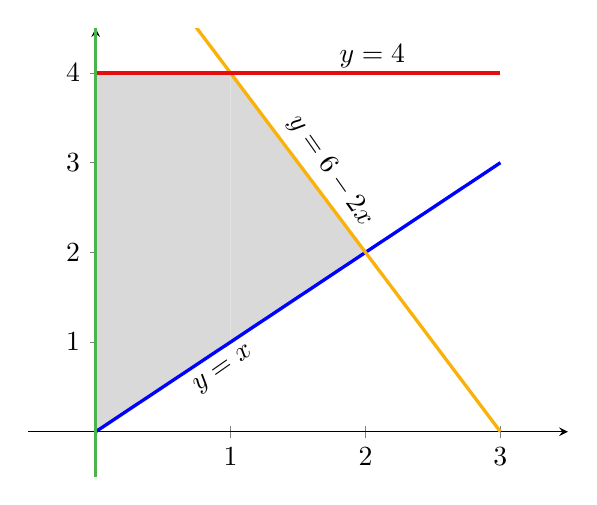
\begin{tikzpicture}
\begin{axis}[
axis lines=middle,
xmin=-0.5,xmax=3.5,ymin=-0.5,ymax=4.5
]
\addplot[very thick,blue, samples=300, domain=0:3, name path=A] {x}; 
\addplot[very thick,yellow!70!red, samples=300, domain=0:3, name path=B] {6-2*x}; 
\addplot[very thick,red!90!teal, samples=300, domain=0:3, name path=C] {4}; 
\addplot[very thick,green!70!magenta, samples=300, domain=0:3, name path=D] coordinates{(0,-6) (0,6)};
\addplot[gray!30] fill between[of=A and C,soft clip={domain=0:1}];
\addplot[gray!30] fill between[of=A and B,soft clip={domain=1:2}];
\node [rotate=35] at (axis cs:  0.95,  .69) {$y=x$};
\node [rotate=-55] at (axis cs:  1.74,  2.91) {$y=6-2x$};
\node [rotate=0] at (axis cs:  2.05,  4.19) {$y=4$};
\end{axis}
\end{tikzpicture}

\begin{parts}
	\part[3] \label{part:one} One of the corner points of the feasible region is $(0,0)$. Find the other three corned points. Show Your work step by step and include explanations.
	\fillwithdottedlines{4cm}
	\bonuspart[1]  (Circle the one correct answer.) The feasible region shown above is:
	\begin{oneparchoices}
		\choice bounded; 
		\choice unbounded.
	\end{oneparchoices}
	
	\part[4] Find the maximum value of the objective function $10-4x+2y$ in the feasible region shown above. Please use the method described in class to solve this problem and show your work step by step.
	\fillwithdottedlines{4cm}
\end{parts}	

\question[1] A function $f$ is given below, and the indicated transformations are applied to its graph (in the given order). Write the equation for the final transformed graph.
\smallskip

$f(x) = |x|$;
reflect in the $x$-axis, then shift 3 units to the right, then shift upward 2 units.

\fillwithdottedlines{2cm}
\newpage
\question[2] \label{question:one} On the grid provided below, draw the graph of a function $f$ with all of the following properties:

\begin{minipage}[t][][b]{0.5\textwidth}
	\begin{multicols}{2}
		\begin{enumerate}
			\item The domain of $f$ is $[2,5]$;
			\item The range of $f$ is $[1,4]$;
			\item $f(2)=1$;
			\item The function {\bf{is}} one-to-one.
		\end{enumerate}
	\end{multicols}
	(Note: don't forget to draw and label the axes, and include units.)
\end{minipage}
\begin{minipage}[t][][b]{0.5\textwidth}
	\begin{center}
		
\begin{tikzpicture}
		\draw[gray!50, thin, step=0.5] (0,-2) grid (6,2);
		\end{tikzpicture}
	\end{center}
\end{minipage}	
\bonusquestion[1] (This question refers to the graph of the function $f$, which You sketched in Question~\ref{question:one}) Find $f(5)$. %\dotfill
\fillwithdottedlines{1cm}
%\smallskip

\bonusquestion[2]  Draw a possible graph of a polynomial $P(x)$ of even degree, with exactly two $x$-intercepts, $(1,0)$ and $(3,0)$, and such that the graph bounces off the $x$-axis at $(1,0)$ and $(3,0)$. [Note: no credit given for a graph where units are not included.]
\smallskip\fillwithgrid{1.8in}
%\begin{tikzpicture}[thick,scale=0.9, every node/.style={scale=0.6}]

%\draw[gray!70, thin, step=0.5] (-1,-3) grid (\linewidth-\pgflinewidth,3);

%\end{tikzpicture}

\question This question has\setcountertopartsofq{\arabic{question}}
\underline{\wordnum{numpofq}} (\arabic{numpofq}) parts
((a)---(\alph{numpofq})).

  Variable stars are ones whose brightness varies periodically. The brightness of a certain star is modeled by the function
$\displaystyle b(t) = 8.8 - 2.7 \cos \left (\frac{\pi}{154}t\right )$ where $t$ is measured in days.'
\begin{parts}
	\part[2] Find the period. 
	\fillwithdottedlines{0.8in}
	\part[2]Find the  minimum brightness. 
	\fillwithdottedlines{0.8in}
\end{parts}
\newpage

\question This question has\setcountertopartsofq{\arabic{question}}
\underline{\wordnum{numpofq}} (\arabic{numpofq}) parts
((a)---(\alph{numpofq})).

A Ferris wheel with 59 capsules has a diameter of 110 meters and its lowest point (at the 6 o'clock position) is 5 meters above the ground. One full rotation of the wheel takes 24 minutes, and the wheel rotates counterclockwise at a constant speed. The capsules are labeled from 1 to 59. We start observing when capsule 1 is at the lowest point on the wheel. Let $H(t)$ be the height of capsule 1 $t$ minutes after we start the observation. 

\begin{parts}

			\part[2] Write the equation of $H(t)$ using the sine function, that is, write $H(t)$ as $\displaystyle a\sin(B(x-h))+k$.
			\fillwithdottedlines{2cm}
			
			\part[2] Find the exact times when capsule 1 is at a height of 80 meters during the first rotation ($0\leq t \leq 24$).
			
			\fillwithdottedlines{3.5cm}
			\part[1] If we restrict the domain of $H$ to the first half of the first rotation ($0\leq t \leq 12$) then the function $H$ becomes one-to-one. The units of the number \enquote{70} in $\displaystyle H^{-1}(70)$ are: \begin{oneparchoices}
				\choice meters; \choice seconds. 
			\end{oneparchoices}	
					\part[4] Let's consider two more Ferris wheels (call them Ferris wheels 2 and 3), each with 59 evenly spaced capsules. The height from the ground of capsule 1 in Ferris wheel 2 is given by $H(2t)$, while the height from the ground of capsule 1 in Ferris wheel 3 is given by $H(t)+2$. 
					\begin{enumerate}
						\item The lowest point of Ferris wheel 2 from the ground is:
						\fillwithdottedlines{1.5cm} 
						\item The lowest point of Ferris wheel 3 from the ground is:
						\fillwithdottedlines{1.5cm}
						\item Find the time it takes for Ferris wheel 2 to complete one full rotation:
						\fillwithdottedlines{1.5cm}
						\item Find the time it takes for Ferris wheel 3 to complete one full rotation:
						\fillwithdottedlines{1.5cm}	
					\end{enumerate}	
	\end{parts}

\newpage
 			

\question[2] Find the exact solution of the equation: $\displaystyle 2e^{-x}=19$.

\fillwithdottedlines{1.5cm}

\question[2] Find the exact solution of the equation: $\displaystyle \log(x) + \log(x - 3) = \log(3x)$.

\fillwithdottedlines{2cm}

 \question[2] Write the exact values of the two solutions of the equation $\displaystyle \sin x = 0.4$ in $[0,2\pi]$.
 
 \fillwithdottedlines{1.5cm}
 
 \question[2] The present value of a sum of money is the amount that must be invested now, at a given rate of interest, to produce the desired sum at a later date. 
 
 Find the present value of \$10,000 if interest is paid at a rate of 0.1\% per year, compounded daily, for 2 years. Write Your answer in exact form.
 
 \fillwithdottedlines{2cm}
 
 \question[2] A quantity, called Quantity A, starts at a size of 100 units (at $t=0$ minutes) and grows exponentially. After 1 minute, the size of Quantity A is 101 units. Find the number of minutes it takes for Quantity A to double.    Show all Your work step-by-step and give Your answer in exact form. Note: You do not have to provide a decimal approximation of Your answer.
 
 
 \fillwithdottedlines{2cm}
 
 \question[2] Another quantity, called Quantity B, starts at a size of 100 units (at $t=0$ minutes) and decreases exponentially. After 1 minute, the size of Quantity A is 99 units. Find the number of minutes it takes for Quantity B to reach a size of 50 units.     Show all Your work step-by-step and give Your answer in exact form. Note: You do not have to provide a decimal approximation of Your answer.
 
 \fillwithdottedlines{2cm}
\bonusquestion[1] The function $\displaystyle f(x)=\frac{2x-1}{(x+1)(2x-1)}$ has two distinct vertical asymptotes. 
\begin{oneparchoices}
\choice True \choice False
\end{oneparchoices}

\bonusquestion[1]
 True or False? If the statement is always true, write True in the space provided below; otherwise, write False.
 $\displaystyle \sin^{-1}\left ( \sin \left ( 11\frac{\pi}{4}\right ) \right ) = -\frac{\pi}{4}$ \dotfill
 
 
 
 
 \question[2] The size of a population $P$ is given by the function: $\displaystyle P(t)=200(1+2e^{-0.18t})$. Find the initial size of the population. Show all Your work step-by-step.
 
 \fillwithdottedlines{2cm}
 
 		\question This question has\setcountertopartsofq{\arabic{question}}
 		\underline{\wordnum{numpofq}} (\arabic{numpofq}) parts
 		((a)---(\alph{numpofq})).
 		
 		Find the exact value of each of the quantities listed below. If a quantity is undefined, please write DNE as Your answer.
 		
 		\begin{parts}
 			\begin{multicols}{2}
 				\part[1] $\displaystyle \sin \left ( -\frac{17\pi}{4} \right ) $ \dotfill
 				\part[1] $\displaystyle \sin^{-1} \left ( -\frac{17\pi}{4} \right ) $ \dotfill
 				\bonuspart[1] $\displaystyle \cos\left (\frac{\pi}{2}\right )$ \dotfill
 				\bonuspart[1] $\displaystyle \sin \left (-\frac{\pi}{2}\right )$ \dotfill
 				\part[1] $\displaystyle \sin^{-1}\left (-\frac{\sqrt{3}}{2}\right )$ \dotfill
 				\part[1] $\displaystyle \cos^{-1}\left (-\frac{\sqrt{3}}{2}\right )$ \dotfill	
 			\end{multicols}
 		\end{parts}	
 		
 		\question This question has\setcountertopartsofq{\arabic{question}}
 		\underline{\wordnum{numpofq}} (\arabic{numpofq}) parts
 		((a)---(\alph{numpofq})).
 		
 		True or False? If a statement is always true, write True in the space provided below; otherwise, write False.
 		\begin{parts}
 			\begin{multicols}{2}
 				
 				\part[1] $\displaystyle \frac{\log x}{\log y}=\log \left (\frac{x}{y}\right )$ \dotfill
 				
 				\part[1] $\displaystyle \left(\log \left( x\right)\right)^2=2\left(\log \left( x\right)\right)$\dotfill
 				
 				\part[1]  $\displaystyle \log_2 \left( \frac{1}{2} \right) = -1$ \dotfill
 				
 				\part[1]  $\displaystyle \log(0)=1$ \dotfill
 				
 				\part[1] $\displaystyle \log(0.001)=-3$ \dotfill
 				
 				\part[1] $\displaystyle \log(100)=2$ \dotfill
 				
 			\end{multicols}
 		\end{parts}	
 		
 		\question[3] One and a half period of the graph of a function $\displaystyle f(x)=a\cos(b(x-h))$ is shown below.
 	\begin{minipage}[t][][b]{0.5\textwidth}	
 		\begin{center}
 			
 			\begin{mfpic}[25]{-2}{6}{-3}{4}
 				\point[3pt]{(-1,3),  (1,-3),  (3,3),(5,-3)}
 				\tlabel(-2.25,3.35){\tiny $\left(-1,3\right)$}
 				%\tlabel(0.75,0.35){\tiny $\left(\frac{1}{2},\frac{1}{2}\right)$}
 				\tlabel[cc](1,-3.35){\tiny $\left(1,-3\right)$}
 				%\tlabel(3.75,0.35){\tiny $\left(\frac{7}{2},\frac{1}{2}\right)$}
 				\tlabel(3.25,3.35){\tiny $\left(3,3\right)$}
 				\tlabel[cc](5,-3.35){\tiny $\left(5,-3\right)$}
 				\axes
 				\tlabel[cc](6,-0.25){\scriptsize $x$}
 				\tlabel[cc](0.25,4){\scriptsize $y$}
 				%	\tcaption{One period  of $y = f(x)$.}
 				\xmarks{-1,1,2,3,4,5}
 				\ymarks{-2,-1,1,2,3}
 				\tlpointsep{4pt}
 				\axislabels {x}{{\tiny $-1 \hspace{7pt}$} -1, {\tiny $1$} 1,  {\tiny $2$} 2,  {\tiny $3$} 3,  {\tiny $4$} 4,  {\tiny $5$} 5}
 				\axislabels {y}{ {\tiny $-2$} -2,{\tiny $-1$} -1, {\tiny $1$} 1, {\tiny $2$} 2, {\tiny $3$} 3}
 				\dotted \function{-2, -1, 0.1}{3*cos(3.14159265*(x+1)/2)}
 				\dotted \function{5, 6, 0.1}{3*cos(3.14159265*(x+1)/2)}
 				\function{-1, 5, 0.1}{3*cos(3.14159265*(x+1)/2)}
 			\end{mfpic}
 			
 		\end{center}
 	\end{minipage}\begin{minipage}[t][][b]{0.5\textwidth}
 		Find $a,b,c$.
 		%\fillwithdottedlines{3.5cm}
 		\bigskip
 		
 		$a=$ \dotfill
 		\bigskip
 		
 		$b=$ \dotfill
 		\bigskip
 		
 		$h=$ \dotfill
		\end{minipage}		
					\end{questions}
					\newpage
					%\newpage
\par\medskip\hrule\medskip


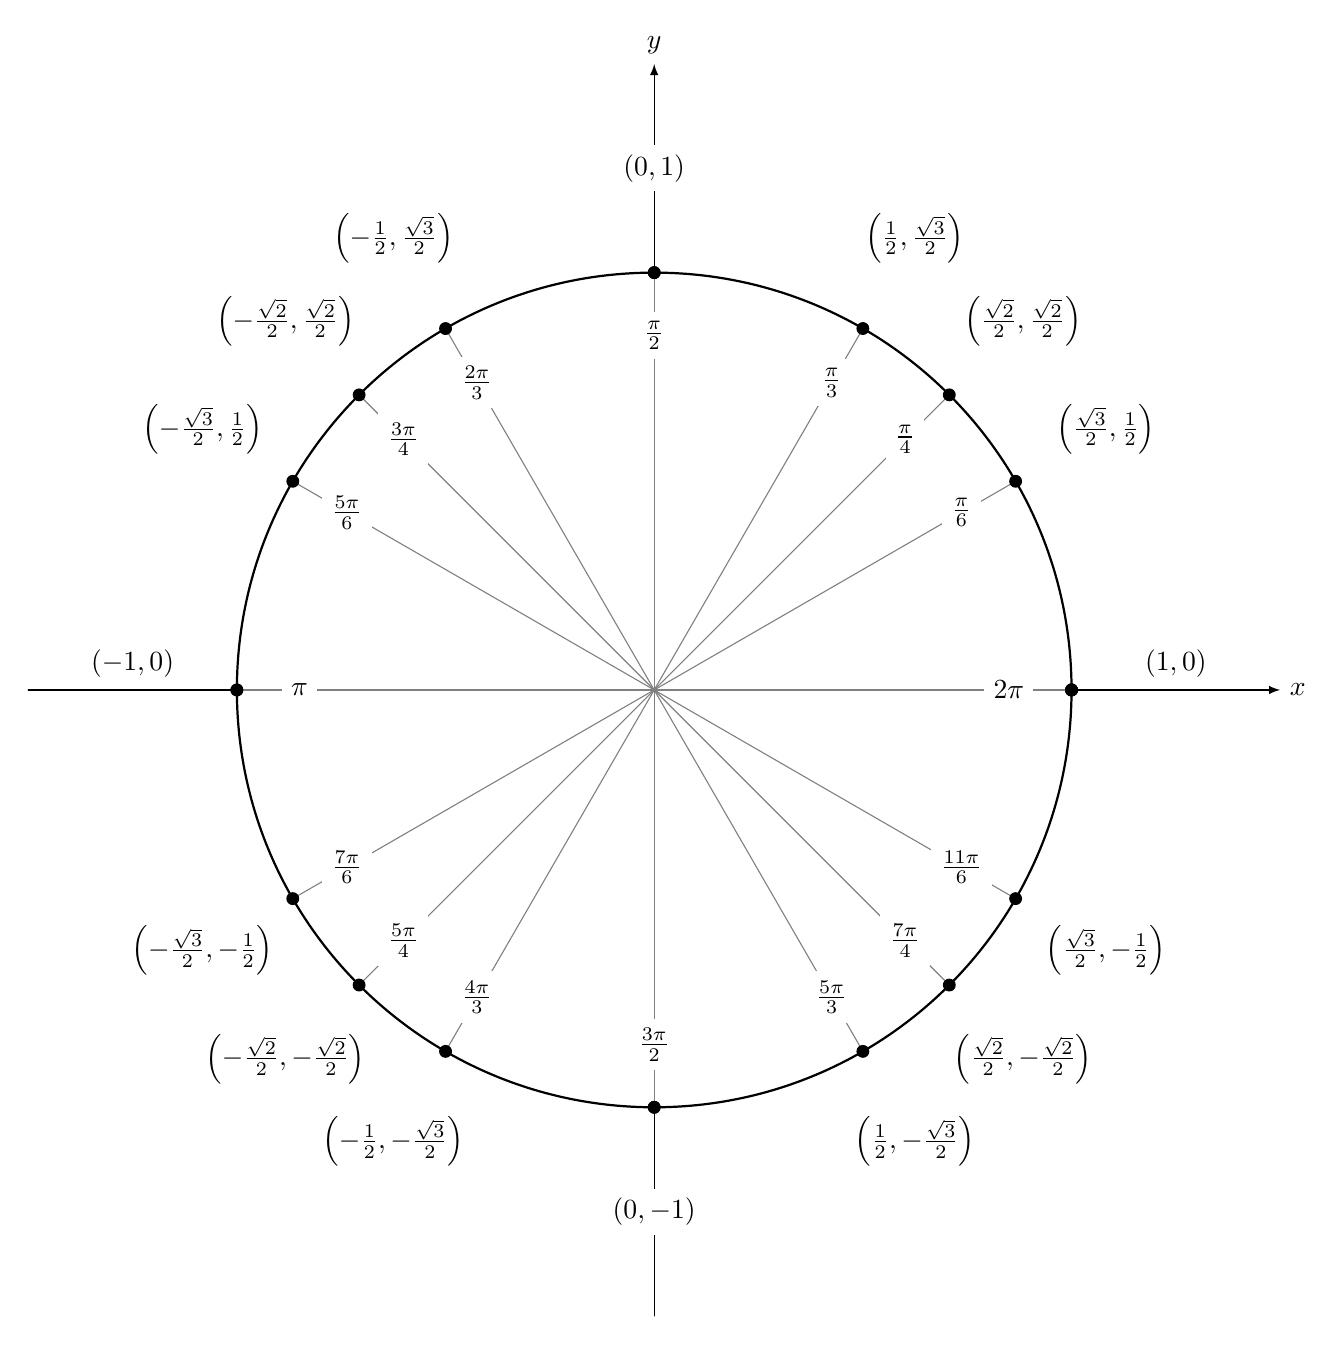
\begin{tikzpicture}[scale=5.3,cap=round,>=latex]
% draw the coordinates
\draw[->] (-1.5cm,0cm) -- (1.5cm,0cm) node[right,fill=white] {$x$};
\draw[->] (0cm,-1.5cm) -- (0cm,1.5cm) node[above,fill=white] {$y$};

% draw the unit circle
\draw[thick] (0cm,0cm) circle(1cm);

\foreach \x in {0,30,...,360} {
	% lines from center to point
	\draw[gray] (0cm,0cm) -- (\x:1cm);
	% dots at each point
	\filldraw[black] (\x:1cm) circle(0.4pt);
	% draw each angle in degrees
	%\draw (\x:0.6cm) node[fill=white] {$\x^\circ$};
}

\foreach \x in {0,45,...,360} {
	% lines from center to point
	\draw[gray] (0cm,0cm) -- (\x:1cm);
	% dots at each point
	\filldraw[black] (\x:1cm) circle(0.4pt);
	% draw each angle in degrees
	%\draw (\x:0.6cm) node[fill=white] {$\x^\circ$};
}
% draw each angle in radians
\foreach \x/\xtext in {
	30/\frac{\pi}{6},
	45/\frac{\pi}{4},
	60/\frac{\pi}{3},
	90/\frac{\pi}{2},
	120/\frac{2\pi}{3},
	135/\frac{3\pi}{4},
	150/\frac{5\pi}{6},
	180/\pi,
	210/\frac{7\pi}{6},
	225/\frac{5\pi}{4},
	240/\frac{4\pi}{3},
	270/\frac{3\pi}{2},
	300/\frac{5\pi}{3},
	315/\frac{7\pi}{4},
	330/\frac{11\pi}{6},
	360/2\pi}
\draw (\x:0.85cm) node[fill=white] {$\xtext$};

\foreach \x/\xtext/\y in {
	% the coordinates for the first quadrant
	30/\frac{\sqrt{3}}{2}/\frac{1}{2},
	45/\frac{\sqrt{2}}{2}/\frac{\sqrt{2}}{2},
	60/\frac{1}{2}/\frac{\sqrt{3}}{2},
	% the coordinates for the second quadrant
	150/-\frac{\sqrt{3}}{2}/\frac{1}{2},
	135/-\frac{\sqrt{2}}{2}/\frac{\sqrt{2}}{2},
	120/-\frac{1}{2}/\frac{\sqrt{3}}{2},
	% the coordinates for the third quadrant
	210/-\frac{\sqrt{3}}{2}/-\frac{1}{2},
	225/-\frac{\sqrt{2}}{2}/-\frac{\sqrt{2}}{2},
	240/-\frac{1}{2}/-\frac{\sqrt{3}}{2},
	% the coordinates for the fourth quadrant
	330/\frac{\sqrt{3}}{2}/-\frac{1}{2},
	315/\frac{\sqrt{2}}{2}/-\frac{\sqrt{2}}{2},
	300/\frac{1}{2}/-\frac{\sqrt{3}}{2}}
\draw (\x:1.25cm) node[fill=white] {$\left(\xtext,\y\right)$};

% draw the horizontal and vertical coordinates
% the placement is better this way
\draw (-1.25cm,0cm) node[above=1pt] {$(-1,0)$}
(1.25cm,0cm)  node[above=1pt] {$(1,0)$}
(0cm,-1.25cm) node[fill=white] {$(0,-1)$}
(0cm,1.25cm)  node[fill=white] {$(0,1)$};
\end{tikzpicture}	
					
					
					\newpage
					
					
					\thispagestyle{empty}
					
					
					\setlength\fboxrule{2pt}\setlength\fboxsep{2mm}
					\fbox{This page is intentionally left blank.} You may use it as scrap paper for your calculations.
				\end{document}                 